\documentclass{book}

\usepackage[utf8]{inputenc}
\usepackage[T1]{fontenc}
\usepackage{lmodern}
\usepackage[a4paper,width=138mm,top=35mm,bottom=35mm,bindingoffset=10mm]{geometry}
\usepackage{url}
\usepackage{titlesec}
\usepackage{graphicx}
\usepackage{hyperref}
\usepackage{rotating}
\usepackage{listings}
\usepackage{pdflscape}
\usepackage{mathrsfs,amsmath}
\usepackage{units}
\usepackage{siunitx}
\usepackage{acronym}
\usepackage{booktabs}
\usepackage{bibentry}
\usepackage{subcaption}
\usepackage{natbib}
\usepackage[export]{adjustbox}
\usepackage{amsmath}
\usepackage{amssymb}
\usepackage{chemfig}
\usepackage{mathtools}
\usepackage{listings}
\usepackage{wrapfig}
\usepackage{color}
\usepackage{float}
\usepackage{caption}
\usepackage{paralist}
\usepackage{tcolorbox}
\usepackage{braket}
\usepackage[framemethod=TikZ]{mdframed}
\usepackage[english]{babel}
\usepackage{esint}
\usepackage{hyperref}

\title{Exploit Notebook}
\date{2020-01-01}
\author{Kalp Shah}

\lstdefinestyle{shared}{
    belowcaptionskip=1\baselineskip,
    breaklines=true,
    xleftmargin=\parindent,
    showstringspaces=false,
    basicstyle=\fontsize{10}{6}\ttfamily,
}
\lstdefinestyle{cpp}{
	style=shared,
    language=C++,
    keywordstyle=\bfseries\color{green!40!black},
    commentstyle=\itshape\color{red!80!black},
    identifierstyle=\color{blue},
    stringstyle=\color{purple!40!black},
}
\lstdefinestyle{java}{
    style=shared,
    language=Java,
    keywordstyle=\bfseries\color{green!40!black},
    commentstyle=\itshape\color{purple!40!black},
    identifierstyle=\color{blue},
    stringstyle=\color{orange},
}
\lstdefinestyle{py}{
    style=shared,
    language=Python,
    keywordstyle=\bfseries\color{green!40!black},
    commentstyle=\itshape\color{purple!40!black},
    identifierstyle=\color{blue},
    stringstyle=\color{orange},
}
\lstdefinestyle{txt}{
    style=shared,
}
\lstset{escapechar=@}

\newcounter{theo}[section]\setcounter{theo}{0}
\renewcommand{\thetheo}{\arabic{section}.\arabic{theo}}
\newenvironment{theorem}[2][]{%
\refstepcounter{theo}%
\ifstrempty{#1}%
{\mdfsetup{%
frametitle={%
\tikz[baseline=(current bounding box.east),outer sep=0pt]
\node[anchor=east,rectangle,fill=blue!20]
{\strut Theorem~\thetheo};}}
}%
{\mdfsetup{%
frametitle={%
\tikz[baseline=(current bounding box.east),outer sep=0pt]
\node[anchor=east,rectangle,fill=blue!20]
{\strut Theorem~\thetheo:~#1};}}%
}%
\mdfsetup{innertopmargin=10pt,linecolor=blue!20,%
linewidth=2pt,topline=true,%
frametitleaboveskip=\dimexpr-\ht\strutbox\relax
}
\begin{mdframed}[]\relax%
\label{#2}}{\end{mdframed}}


\newcounter{prf}[section]\setcounter{prf}{0}
\renewcommand{\theprf}{\arabic{section}.\arabic{prf}}
\newenvironment{proof}[2][]{%
\refstepcounter{prf}%
\ifstrempty{#1}%
{\mdfsetup{%
frametitle={%
\tikz[baseline=(current bounding box.east),outer sep=0pt]
\node[anchor=east,rectangle,fill=red!20]
{\strut Proof~\theprf};}}
}%
{\mdfsetup{%
frametitle={%
\tikz[baseline=(current bounding box.east),outer sep=0pt]
\node[anchor=east,rectangle,fill=red!20]
{\strut Proof~\thetheo:~#1};}}%
}%
\mdfsetup{innertopmargin=10pt,linecolor=red!20,%
linewidth=2pt,topline=true,%
frametitleaboveskip=\dimexpr-\ht\strutbox\relax
}
\begin{mdframed}[]\relax%
\label{#2}}{\end{mdframed}}


\newcounter{prob}[section]\setcounter{prob}{0}
\renewcommand{\theprob}{\arabic{section}.\arabic{prob}}
\newenvironment{problem}[2][]{%
\refstepcounter{prob}%
\ifstrempty{#1}%
{\mdfsetup{%
frametitle={%
\tikz[baseline=(current bounding box.east),outer sep=0pt]
\node[anchor=east,rectangle,fill=red!80]
{\strut Problem~\theprob};}}
}%
{\mdfsetup{%
frametitle={%
\tikz[baseline=(current bounding box.east),outer sep=0pt]
\node[anchor=east,rectangle,fill=red!80]
{\strut Problem~\theprob:~#1};}}%
}%
\mdfsetup{innertopmargin=10pt,linecolor=red!80,%
linewidth=2pt,topline=true,%
frametitleaboveskip=\dimexpr-\ht\strutbox\relax
}
\begin{mdframed}[]\relax%
\label{#2}}{\end{mdframed}}


\newcounter{exm}[section]\setcounter{exm}{0}
\renewcommand{\theexm}{\arabic{section}.\arabic{exm}}
\newenvironment{example}[2][]{%
\refstepcounter{exm}%
\ifstrempty{#1}%
{\mdfsetup{%
frametitle={%
\tikz[baseline=(current bounding box.east),outer sep=0pt]
\node[anchor=east,rectangle,fill=green!20]
{\strut Example~\theexm};}}
}%
{\mdfsetup{%
frametitle={%
\tikz[baseline=(current bounding box.east),outer sep=0pt]
\node[anchor=east,rectangle,fill=green!20]
{\strut Example~\thetheo:~#1};}}%
}%
\mdfsetup{innertopmargin=10pt,linecolor=green!20,%
linewidth=2pt,topline=true,%
frametitleaboveskip=\dimexpr-\ht\strutbox\relax
}
\begin{mdframed}[]\relax%
\label{#2}}{\end{mdframed}}


\newcounter{def}[section]\setcounter{def}{0}
\renewcommand{\thedef}{\arabic{section}.\arabic{def}}
\newenvironment{definition}[2][]{%
\refstepcounter{def}%
\ifstrempty{#1}%
{\mdfsetup{%
frametitle={%
\tikz[baseline=(current bounding box.east),outer sep=0pt]
\node[anchor=east,rectangle,fill=yellow!20]
{\strut Definition~\thedef};}}
}%
{\mdfsetup{%
frametitle={%
\tikz[baseline=(current bounding box.east),outer sep=0pt]
\node[anchor=east,rectangle,fill=yellow!20]
{\strut Definition~\thedef:~#1};}}%
}%
\mdfsetup{innertopmargin=10pt,linecolor=yellow!20,%
linewidth=2pt,topline=true,%
frametitleaboveskip=\dimexpr-\ht\strutbox\relax
}
\begin{mdframed}[]\relax%
\label{#2}}{\end{mdframed}}

\let\cleardoublepage\clearpage


\begin{document}
\pagenumbering{arabic}

\begin{titlepage}
    \newcommand{\HRule}{\rule{\linewidth}{0.5mm}}
    \center
    \textsc{\LARGE International Institute of Information Technology, Hyderabad}\\[0.5cm]
    
\includegraphics[scale=1]{logo.png}\\[0.5cm]
    \textsc{\Large Information Security}\\[0.5cm]
    \textsc{\large Cryptography, Pwning and Exploit Research}\\[0.5cm] % Minor heading such as course title
    \HRule \\[0.4cm]
    { \huge \bfseries Hacking Handbook}\\[0.4cm]
    \HRule \\[1.5cm]
    \begin{minipage}{0.6\textwidth}
        \begin{flushleft} \large
            \center
            \emph{Author:} Kalp Shah \\
            %\emph{Maintainers:} Animesh Sinha, Gourang Tandon, Yogottam Khandelwal.
        \end{flushleft}
    \end{minipage}\\[2cm]
    {\large \today}\\[2cm]
\end{titlepage}

\section*{Abstract}
A thorough foray into exploitation and explanation of why it
works the way it does. It is a compilation of sorts, and hence no
correlation between chapters (No flow b/w chapters exist) and the
book should exist as a case study and used to solve problems which
look similar and also has some basics which I go learning on the
way forward.
``\emph{If it moves, compile it}''.


\section*{Sources}
The websites and competitions referred for writing this piece:
\begin{itemize}
    \item \href{https://ctf101.org}{CTF 101}
    \item \href{https://shellterlabs.com}{Shellter Labs}
    \item Linux Man Pages
    \item \href{https://picoctf.com}{picoCTF}
    \item \href{https://trailofbits.github.io/ctf}{trailofbits}
    \item \href{http://www.cs.fsu.edu/~redwood/OffensiveComputerSecurity/lectures.html}{Florida University Computer Security}
    \item \href{https://www.megabeets.net/a-journey-into-radare-2-part-1/}{Megabeets Radare Tutorial}
    \item \href{https://developer.android.com/studio/command-line/adb}{Android Developers Website}
\end{itemize}
\vfill

\newpage
% !TEX root = ../thesis.tex
% \pdfbookmark[0]{Acronyms}{Acronyms}
\chapter{Basics}
\section{Data}
There are many places to store data on a typical computer like 
a hard drive ( or any other secondary storage ), RAM, Caches 
and Registers.\\\\A hierarchy is decided on their access speed. 
If a piece of data is required more frequently, it is stored on 
a faster storage device. ( Faster implies lower latency i.e. time 
taken from being asked for data and providing it ). The figure 1 
shows this heirarchy.\\

\begin{figure}
    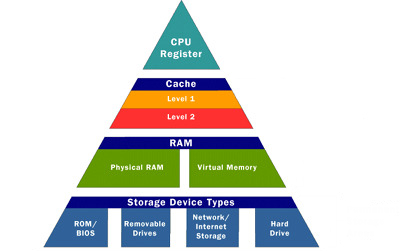
\includegraphics[width = 0.50\textwidth, center]{gfx/storageHierarchy.jpg}    
    \caption{Latency Hierarchy}
\end{figure}

\subsection*{Location}

\subsubsection*{Register}
A register is located in the CPU itself and as it is physically the
closest, it also the fastest. It is the one that is accessed while
running a program\\\\ A sample data flow can be seen in Figure 2, which shows
data tranfer from RAM to Register and then to the CPU.

\begin{figure}
    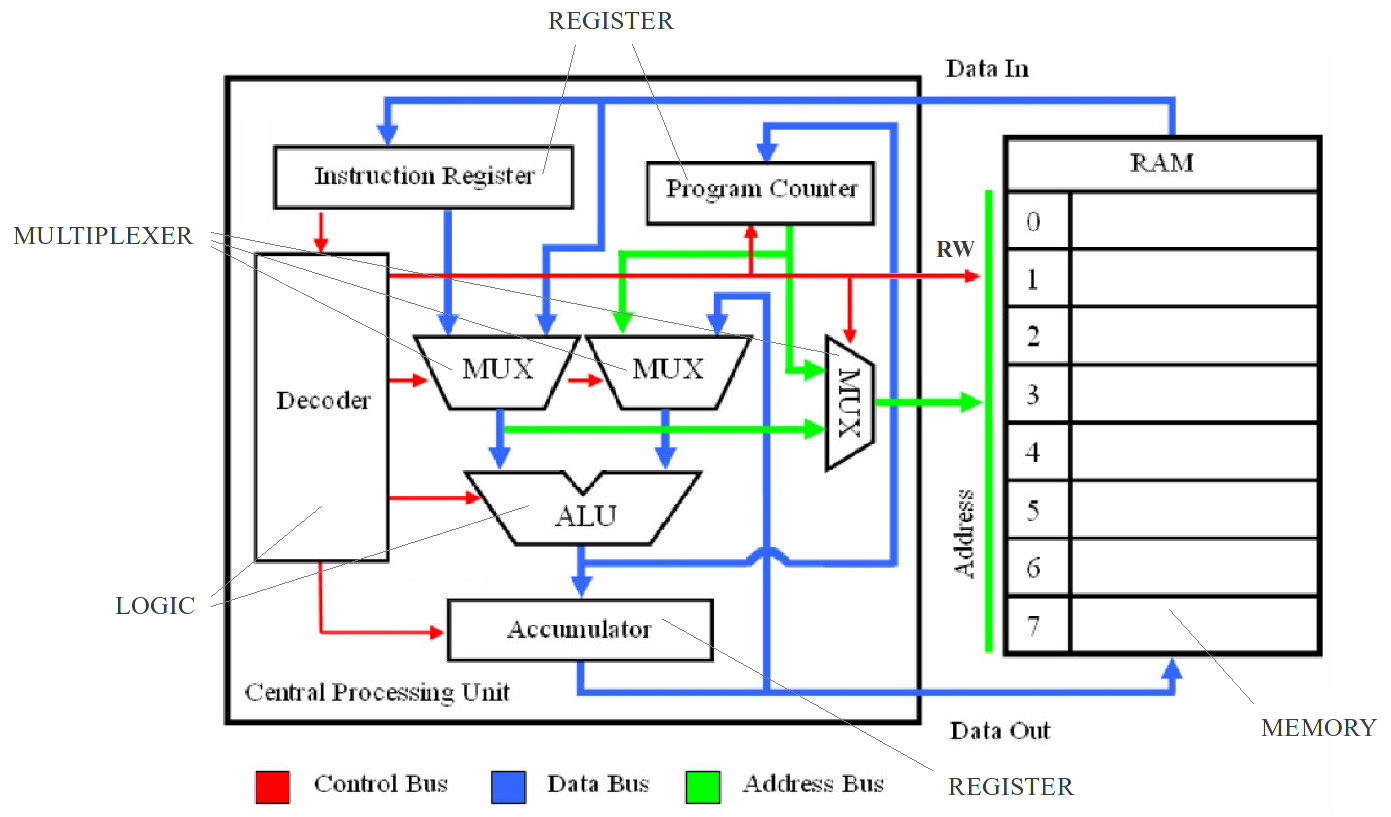
\includegraphics[width = 0.9\textwidth, center]{gfx/cpu.jpg}    
    \caption{Circuit of CPU}
\end{figure}

\subsubsection*{Cache}
A cache is small piece of memory located near the CPU and works as a
faster RAM (sort of). It caches the data which the OS thinks is required 
the most.\\\\L1 \& L2 cache is built into the proccessor (recent ones anyway) 
and is individual for every physical core whereas L3 cache is located
outside of the actual silicon but is in the chip and so is common for 
all cores.

\subsubsection*{RAM}
RAM is a volatile memory where all the memory that is deemed by the 
OS as required is stored for instant access with the CPU. The data 
tranfer happens from RAM $\rightarrow$ Cache $\rightarrow$ Register.

\subsection*{Bridges}
Bridges are small microcontrollers with built in logic which help in 
communication with external devices. There are two of there, and are 
descibed by their position on the board and also the threshold speed 
they can manage.
\subsubsection*{North Bridge}
 North bridge is a controller chip which connect high speed external 
 devices to the chipset. It was originaly outside ot the main chip 
 and an external silicon but now is mostly included in the SoC ( System on
 a chip ). The devices which can be connected to it are given in 
 Figure 3.

 \begin{figure}
    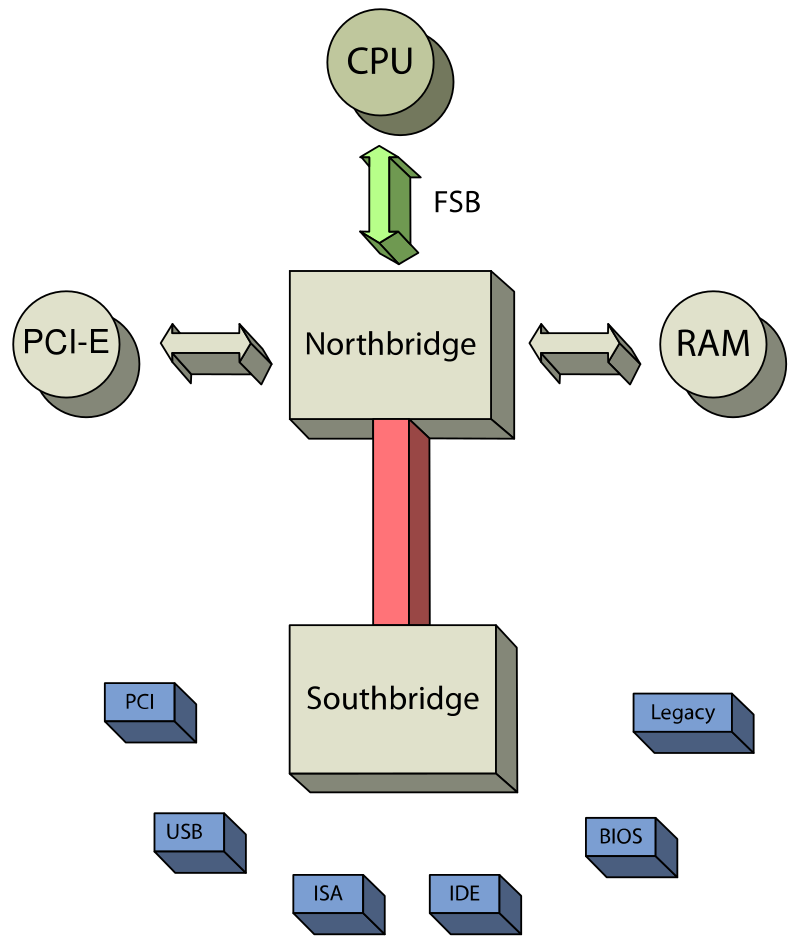
\includegraphics[width = 0.50\textwidth, center]{gfx/ChipSchem.png}    
    \caption{Use of bridges}
\end{figure}

\begin{figure}
    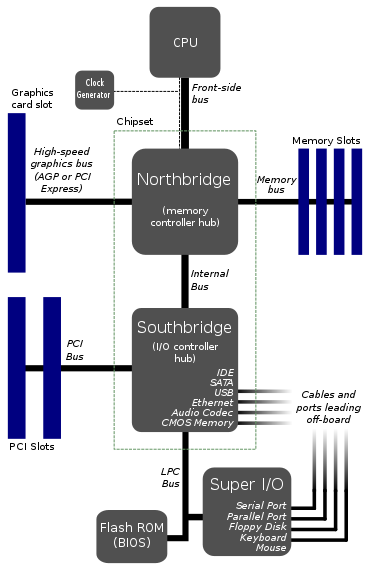
\includegraphics[width = 0.50\textwidth, center]{gfx/Motherboard.png}    
    \caption{Schematic Design of Bridges}
\end{figure}

\subsubsection*{South Bridge}
South bridge is the chipset which connects slower and legacy devices 
to the main chip. It is still seperate on Intel boards but is now 
starting to get integrated in AMD motherboards.

\subsection*{Data Flow}
So the data flow happens as follows :
\begin{center}$Solid\ State \rightarrow South\ Bridge \rightarrow RAM 
\rightarrow Register $
\end{center}
So when a computer is started, it first POSTS and then goes to 
the BIOS after which the BIOS piont the program to the Magic Number 
( For legacy MBR systems ) which has the bootloader in it (Like GRUB), 
after which the bootloader takes control of the System, then loades the 
kernel and with that the OS, which loads itself in the RAM, for fast 
access (The most recently executed programs still in the registers and 
cache) after which the OS loads a GUI ( If it has one ) or just greets 
to a TTY terminal. For the non GUI version, it gets you to a log in 
screen, whicle for GUI an application is loaded which takes care of 
logging in ( Known as a Display Manager (DM) ).

\begin{figure}
    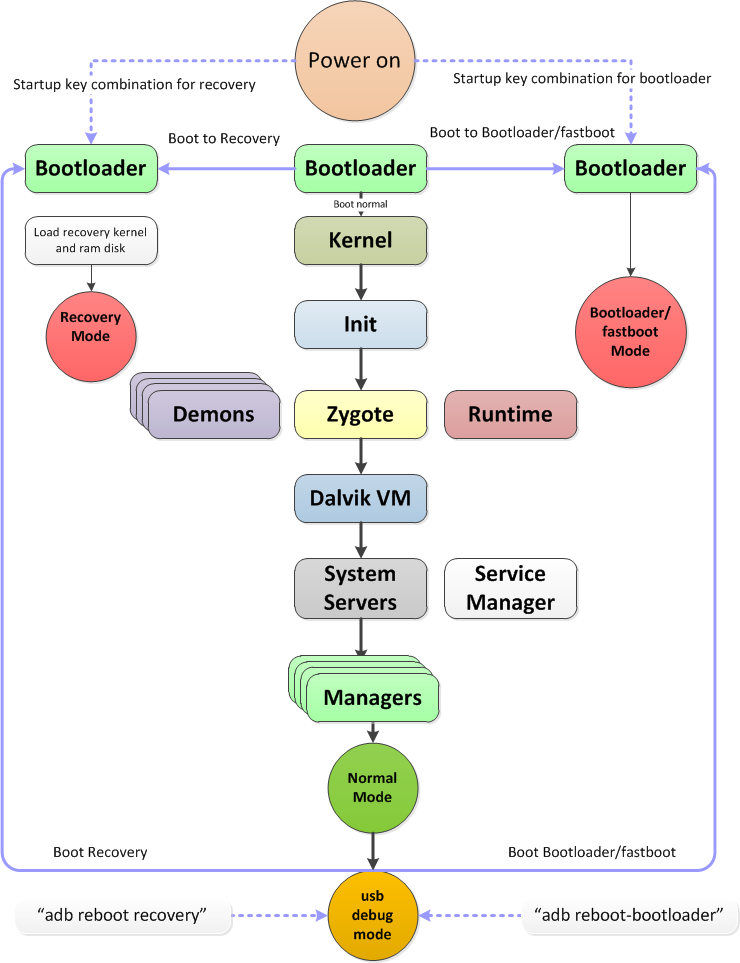
\includegraphics[width = 0.60\textwidth, center]{gfx/android-booting-process.png}    
    \caption{Android booting process}
\end{figure}

% !TEX root = ../thesis.tex
% \pdfbookmark[0]{Acronyms}{Acronyms}
\chapter{Tools}
There are many tools which make analysing and understaing flaws of programs very easy. Most of them are not required and work can be done without them, but they are a good creature comfort and sholud be used as such. These tools are used to analyse a piece of code and understand its vulnerabilites and also to  generate payloads to make exploiting them easier.

\section{GDB}
GDB is one of the most importatnt tools. It is one of, if not the most importatnt tool for exploiting binaries. It is essentially a debugger which allows for dissasmbly of binaries, is also usefull for checking the flow of the the binary, and before Ghidra was one of the most popular tools to understand the working of a program. It is still used for basic analysis, to check if the exploit works, and for initial routing checking. If someone is starting out with binary exploitation, then that someone should exclusively use GDB till the fundamentals of exploitation done are understood.

\subsection*{Basic Setup}
GDB is usually pre installed on any linux machine. But if it isn't, it can be installed using the default package manager ( Like apt or pacman ). There are some extensions for GDB that make it a much easier tool to operate with. You can use any number of them to make it to your liking, but in the following section, only some extensions are used and explained.

\section{radare2}
Radare is a tool which helps in understanding the binary, decompiling 
it and allowing to modify commands on the fly. It is considered one of 
the most difficult tools to master, so much so, that they themselves 
put Figure 6 on their website. I think this can be the Maya of exploiation 
tools.

\begin{figure}
    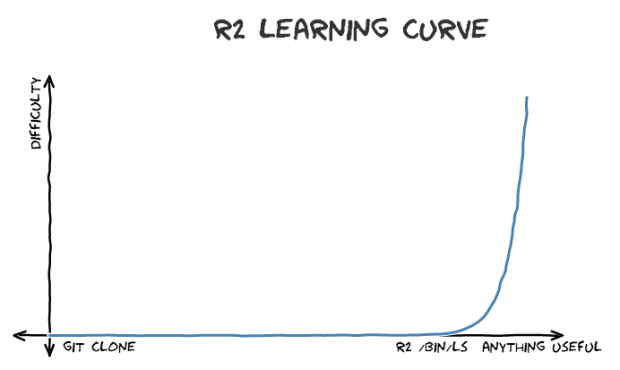
\includegraphics[width = 0.50\textwidth, center]{gfx/radare_learning.png}    
    \caption{Radare Learning Curve}
\end{figure}
\mainmatter
\chapter{Encryption and Decryption Techniques}



\section{Overview}
Cryptography is traditionally associated with opening a message with a key, which is only known by the parties in the communication and no once else.\\\\
This was true at that time and in some sense still is, but nowadays any form of data ( or information ) is protected with a cipher which helps in its secure transmission. Hence the definition has changed over the years.

\begin{definition}[Cryptography]
    It is the practice and study of techniques for secure communication in the presence of third parties called adversaries
\end{definition}

\noindent From the above definition, it can clearly be seen how much it has changed over the years. This should be kept in mind when studying cryptography.

\subsection{Uses}
There are many examples where cryptography is used. It is almost as if every technology that exists wants to protect their information.

\begin{example}
    FFor all types of communication via web, cryptography is used.
    \begin{itemize}
        \item Web Traffic : HTTPS Protocol
        \item Wireless Traffic
              \begin{itemize}
                  \item WiFi Traffic : 802.11 a/b/g/n
                  \item Telephone Signal : GSM
              \end{itemize}
    \end{itemize}
\end{example}

\begin{example}
    EEFS file encryption and Truecrypt are used for protection of files.
\end{example}

\begin{example}
    FFor content protection (DVDs and CDs with copyright media) these technologies are used:
    \begin{itemize}
        \item CSS: Content Scrambling System ( Easily broken )
        \item AACS: Advanced Access Content System ( Not that easy)
    \end{itemize}
\end{example}

\noindent These are some of the examples of how cryptography is used everywhere. Hence understanding them is very important, and so is knowing how vulnerable they are. This can be the difference between building a robust system with good security and one which is easily exploited.



\section{Historical Ciphers}
In this chapter, historical ciphers will be explored. This is the time period where technology and digital communication were not prevalent, and hence these will be a product of the time when they were developed.


\subsection{Substitution Cipher}
This is one of the simplest ciphers that exists. It uses a 26 byte key which is a map from set of alphabets to itself.

\begin{definition}
    Mathemtical definition of the substitution cipher is as follows :\\

    \indent G : Set of ASCII Characters\\
    \indent $f : G \rightarrow G$, $f$ is bijective, such that\\
    \indent $f(\alpha) = \beta$\\

    \noindent$f \rightarrow$ Substitution\ Cipher
\end{definition}

\noindent As it can be seen, the substitution cipher is a hash table, which stores the mapping of every character.

\subsubsection{Code}
This is a sample code on how the substitution cipher encodes. In this only small alphabets are taken into consideration.\\

\lstinputlisting[basicstyle=Large,style=py]{code/ciphers/substitution_encoder.py}


\subsection{Rot - X}
There is a keyless version of the substitution cipher which is an even simpler version of the original cipher. In this, instead of a random key table, here it is a rotation by X (an integer), around which the alphabets are wrapped.

\begin{definition}
    aMathemtical definition of the Rot-X cipher is as follows :\\

    \indent G : Set of ASCII Characters\\
    \indent $f : G \rightarrow G,$\\
    \indent $f(\alpha) = (\alpha + X)\ mod\ 26 $\\

    \noindent$f \rightarrow$ Rot-X\ Cipher
\end{definition}

\subsubsection{Code}
A sample code is written for it, even though it is not required. But well here it is:

\lstinputlisting[basicstyle=Large,style=py]{code/ciphers/rotx_encoder.py}


\subsection{Caesar Cipher}
A Rot-3 cipher is known as a Caesar cipher. This cipher does not even have a key, and hence is technically not a cipher, but came before the generalization Rot-X and hence was widely used at some point in time and still is used as an introduction to ciphers in CTFs.

\subsubsection{Breaking the Cipher}
This is one of the easiest ciphers to break. It is done using a method known as frequency analysis.

\begin{definition}
    Frequency analysis is the study of letters or groups of letters contained in a ciphertext in an attempt to partially reveal the message.
\end{definition}

\noindent So using frequency analysis, the frequency of letters is done on the ciphertext and is mapped to what is standard for the English language and hence the plaintext known by replacing the letters with their maps. \\\\
Here is an example to clear the doubts :

\begin{example}
    dLet us take ciphertext (c) be :
    \begin{verbatim}
LIVITCSWPIYVEWHEVSRIQMXLEYVEOIEWHRXEXIPFEMVEWHKVSTYLXZIXLIKI
IXPIJVSZEYPERRGERIMWQLMGLMXQERIWGPSRIHMXQEREKIETXMJTPRGEVEKE
ITREWHEXXLEXXMZITWAWSQWXSWEXTVEPMRXRSJGSTVRIEYVIEXCVMUIMWERG
MIWXMJMGCSMWXSJOMIQXLIVIQIVIXQSVSTWHKPEGARCSXRWIEVSWIIBXVIZM
XFSJXLIKEGAEWHEPSWYSWIWIEVXLISXLIVXLIRGEPIRQIVIIBGIIHMWYPFLE
VHEWHYPSRRFQMXLEPPXLIECCIEVEWGISJKTVWMRLIHYSPHXLIQIMYLXSJXLI
MWRIGXQEROIVFVIZEVAEKPIEWHXEAMWYEPPXLMWYRMWXSGSWRMHIVEXMSWMG
STPHLEVHPFKPEZINTCMXIVJSVLMRSCMWMSWVIRCIGXMWYMX
    \end{verbatim}

    \noindent I is the most common letter that appears here. It is known that e is the most common English alphabet, and hence I can be replaced with e. Similarly looking at the most common two letter sequence it is XL which can be replaced with in.\\\\ Going on like this, we can successfully find the substitution, which is as follows:
    \begin{verbatim}
Hereupon Legrand arose, with a grave and stately air, and 
brought me the beetle from a glass case in which it was 
enclosed. It was a beautiful scarabaeus, and, at that time, 
unknown to naturalists—of course a great prize in a scientific 
point of view. There were two round black spots near one 
extremity of the back, and a long one near the other. The 
scales were exceedingly hard and glossy, with all the 
appearance of burnished gold. The weight of the insect was 
very remarkable, and, taking all things into consideration, 
I could hardly blame Jupiter for his opinion respecting it.
    \end{verbatim}

    \noindent For more in depth solution, go to :
    \href {https://en.wikipedia.org/wiki/Frequency_analysis#An_example}{Frequency Analysis Wiki}
\end{example}

\subsubsection{Code}
Code for the frequency analysis tool is taken from
\href{https://github.com/CodeDrome/frequency-analysis-python}{CodeDrome} :\\

\lstinputlisting[basicstyle=Large,style=py]{code/ciphers/frequency_analysis.py}

\subsubsection{Working}
The code above initially makes a frequency analysis dictionary with the help of a language text (preferably large), after which it stores it in a JSON. Then that dictionary is used to decode an encoded ciphertext.


\subsection{Vigenère Cipher}
Vigenère Cipher is one of the more competent of the ciphers created by Blaise de Vigenère, who was a French cryptographer. In this cipher, the key is repeated till its size is equal to that of the message. After which it is added to message alphabet by alphabet.

\begin{definition}
    dDefinition of Vigenère Cipher :\\\\
    \indent Pad key till length(key) = length(message)\\
    \indent ciphertext = key $+_{26}$ message
\end{definition}

\noindent In this the key is padded to make it equal to the length of the message. Hence, the key length cannot be greater than that of the cipher (It can be, but won't affect the working of the cipher).

\begin{example}
    lLets take an example of the cipher, to know how it works.\\
    \begin{verbatim}
        key = 'mykey'
        message = 'plztransferthis'    
        len(key) != len(message)
        
        padded_key = 'mykeymykeymykey'
        message    = 'plztransferthis'
        --------------------------------  + mod 26
        ciphertext = 'bjjxpmlcjcdrrmq'
    \end{verbatim}
\end{example}

\subsubsection{Code}
Now that the working of the cipher is known, here is a code for the same:

\lstinputlisting[basicstyle=Large,style=py]{code/ciphers/vigenere_encoder.py}

\subsubsection{Breaking the Cipher}
Start with the assumption that the length of the key is known. Let it be $l$. Hence, in the ciphertext every $l^{th}$ character is coded by the same letter. Therefore, the ciphertext formed from this is a Rot-X.
\\\\
This can be solved using frequency analysis. So the X is now known, the character representation of that X is a letter of the key. Do this for every $l$ letters till the complete key is found, after which the cipher can be decoded.
\\\\
In this, an assumption was made that the length of the key was known, which is not the case. So, start with  $l = 1$, till a comprehendible message is found.

\subsubsection{Code}
This is the code that solves the Vigenère cipher, which is taken from the \href{https://github.com/alpha-k911/Vigenere-Cipher-Decrypter}{alpha-k911 github}.\\

\lstinputlisting[basicstyle=Large,style=py]{code/ciphers/vigenere_decoder.py}


\subsection{Rotor Machines}
During the renaissance, motors were name of the game. So naturally, people wanted to use it in a cipher scheme. Due to that a rotor machine cipher was formed.
\\\\
One of the earlier and simpler rotor machine was the Hebern machine. It has a single rotor and hence encodes a simple 'rotating' substitution table.

\begin{example}
    So the working of a Hebern machine is explained here. The machine encodes a substitution cipher, whose table moves every time a letter is typed.
    \begin{verbatim}
        N                 V                 .
        K                 N                 V
        P                 K                 N
        T  Letter Typed   P  Letter Typed   K
        O  ------------>  T  ------------>  P
        .                 O                 T
        .                 .                 O
        .                 .                 .
        V                 .                 .

        Hence, if m = 'CCC', 
        then c = 'PKN'
    \end{verbatim}
\end{example}

\noindent This is more complex than the standard substitution cipher as same character is encoded to different character according to position of the rotor. Therefore the definition of a Hebern machine is as follows:\\

\begin{definition}
    tThe definition of the Hebern machine, therefore is :\\

    \indent G : Set of ASCII Characters\\
    \indent $f : G \rightarrow G$, $f$ is bijective, such that\\\\
    \indent $f(\alpha + pos(\alpha)) = \beta$;\\
    \indent $pos(\alpha) \rightarrow$ Index of $\alpha$ in the plaintext
\end{definition}

\subsubsection{Code}
Now that the definition of the Hebern machine is known, this is the code :\\

\lstinputlisting[basicstyle=Large,style=py]{code/ciphers/hebern_encoder.py}

\noindent It seems, as if there is no difference between the code of a substitution cipher and this one, but there is. In this the position of the letter is taken into consideration, thus making it a Hebern machine.


\subsection{Enigma Machine}
One of the most popular rotor machine. This was used by the Germans in the World War 2 for intra-communication. This machine had 3-5 rotors in it which would rotate at different speeds and would thus generate a very complicated (for that time) cipher text which was hard to break. \\\\
This machine was reverse engineered and decrypted by a British mathematician Alan Turing, who is very famously known for the Turing machine and the Church-Turing hypothesis.

\subsubsection{Code}
This is a sample code for Enigma machine. If a more detailed and better understanding for the Enigma code is wanted, it can be found on \href{https://github.com/torognes/enigma}{torognes github}.\\

\lstinputlisting[basicstyle=Large,style=py]{code/ciphers/enigma_encoder.py}

\chapter{CryptoGraphy}


\section{Ciphers and Secrecy}

\begin{definition}[Cipher]{def:cipher}
    A Cipher defined over ($\mathcal{K}$ (Key Space), $\mathcal{M}$ (Message Space), $\mathcal{C}$ (Cipher Space)) is a pair of efficient algorithms (E, D), Encryption algorithm $E: \mathcal{K} \times \mathcal{M} \rightarrow \mathcal{C}$ and Decryption algorithm $E: \mathcal{K} \times \mathcal{C} \rightarrow \mathcal{M}$ such that $D(E(\mathcal{C})) = \mathcal{C}$.
\end{definition}


\subsection{One Time Pad}

\begin{definition}[Perfect Secrecy]{def:perfect-secrecy}
    A Cipher has perfect secrecy iff $\forall(m_1, m_2) \in \mathcal{M}, \; len(m_1) = len(m_2), \; P[E(k, m_1) = c] = P[E(k, m_2) = c], \; k \in \mathcal{K} \text{picked uniformly}, \forall c \in \mathcal{C}$. (i.e. No Cipher Text only attack exists, ciphertext yeild no information about the plain text).
\end{definition}

One-Time pad, i.e. a XOR with a Key is a way to get perfect secrecy. However, here the key length has to be the same as the message length, so it's not very useful (since if you can share the key, just use the same means to share the message). It can be proven that \textbf{any keyspace smaller than message space} cannnot obtain perfect secrecy.


\subsection{Pseudo Random Generator}

Now we try to get a more practical cipher which has a smaller key space. (We can still use the pads, but the key has to be smaller, so we will generate a Larger key from a smaller key, then XOR).

\begin{definition}[Pseudo Random Generator]{def:prg}
    A Pseudo Random Generator is a deterministic algorithm which maps a SEED, which is a binary string of length K, to a much longer binary string of length N, but the function is not predictable. i.e.
    \begin{equation}
        PRG(S) = R, \; R \in \{0, 1\}^n, S \in \{0, 1\}^k
    \end{equation}
\end{definition}

What it means to be predictable is that given the first i bits of the generated string, the i + 1 bit can be determined with probability $\geq 1/2 + \epsilon$. Practically $\epsilon$ is considered to be of the order $1/2^{80}$ (But $1/2^{30}$ is not, since it's likely to happen over 1GB of data). Theoretically, it's unpredictable when the value of $\epsilon$ falls off faster than $1/poly(\lambda)$. 


\subsection{Attacks on the Ciphers}

\subsubsection{Never use Two Time Pad}

If the same key is used more than once, the messages can be XORed and then frequency analysis can yeild info on the messages. Therefore reusing a key in two different streams will be insecure.

MS-PPTP protocol in Windows NT used the same key from Server to Client and Client to Server. Though all the messages from Client were one stream, continuing on the Pseudo Random Generator, and so were all from the Server. But two streams used the same key, and that failed.

\textbf{WEP protocol:} has a lot of errors. IV was a counter (24 bits), and that was concatenated with 104 bit long-term key. 
\begin{figure}
    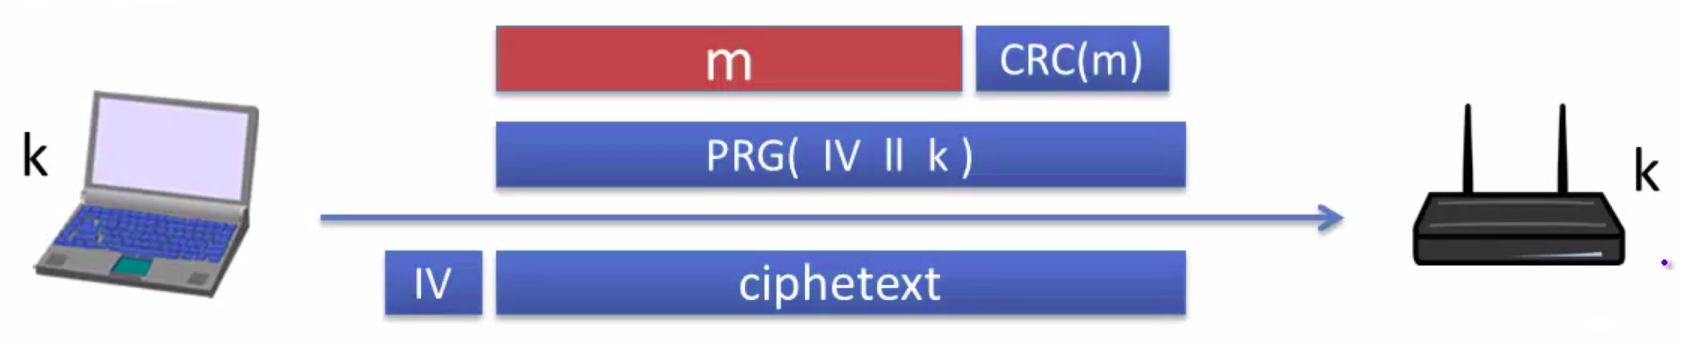
\includegraphics[width = 0.50\textwidth, center]{gfx/crypto/wep-algorithm.png}
    \caption{WEP Protocol}
\end{figure}
After $2^24$ frames, the IV will cycle, so it's like a 2-time pad.
Since the keys only have a counter IV changing every frame, all keys are related, so Due to Shamir, After a 1000000 frames, we can recover the frames, and today even in about 30000 frames. 
The whole stream should have been viewed as a single stream, that would have worked better.

We should also not use this for Disk Encryption, since small changes to the file will change only a few bits. So the before and after edit files are encrypted with same key.

\subsubsection{Integrity Violation}

One Time Pad is malleable, i.e. We can change bits even without encrypting and decrypting. Eg. if we intercept a mail starting with "From: Bob", without knowing the key, we can xor and make it "From: Eve". So the message can be changed.

\subsection{Real World Stream Cipher}

\subsubsection{RC4}
Used in HTTPS and WEP. Weaknesses:
\begin{itemize}
    \item Bias in initial output Pr[2nd Byte] = 2/256
    \item Pr[(0, 0)] = $1/256^2$ + $1/256^3$.
    \item If keys are related, it's possible to recover secret.
\end{itemize}

\subsubsection{CSS}

Linear Feedback Shift Register (LFSR): In every clock cycle, the registers shift by 1, and some bytes are called tap registers, the XOR sum of which gives the results.

CSS has 2 Linear Feedback Shift Register, a 17-bit and a 25-bit LFSR. The Key is 5 bytes. First 2 bytes of key is put into 17-bit LFSR, next 3 bytes in 25-bit LFSR.


\subsection{What is a Secure Cipher}

Since Pseudo Random Generators are deterministic algorithms, and they output numbers uniformly in the space \{0, 1\} in the space .

\begin{equation}
    Advantage_{PRG} [A, G] := |Pr[A(G(k)) = 1] - Pr[A(k) = 1]|
\end{equation}
where k is a random seed, G is the 


\subsubsection{Salsa 20}


XOR encryptions



\section{Block Ciphers}


\subsection{Definitions, DES and AES}

Block ciphers take exactly n-bits of input and map them to exactly n-bits of output.
Some Examples are:
\begin{itemize}
    \item AES, key = 168 bits, n = 64 bits
    \item 3DES, key = 128/192/256 bits, n = 128 bits
\end{itemize}

\begin{figure}
    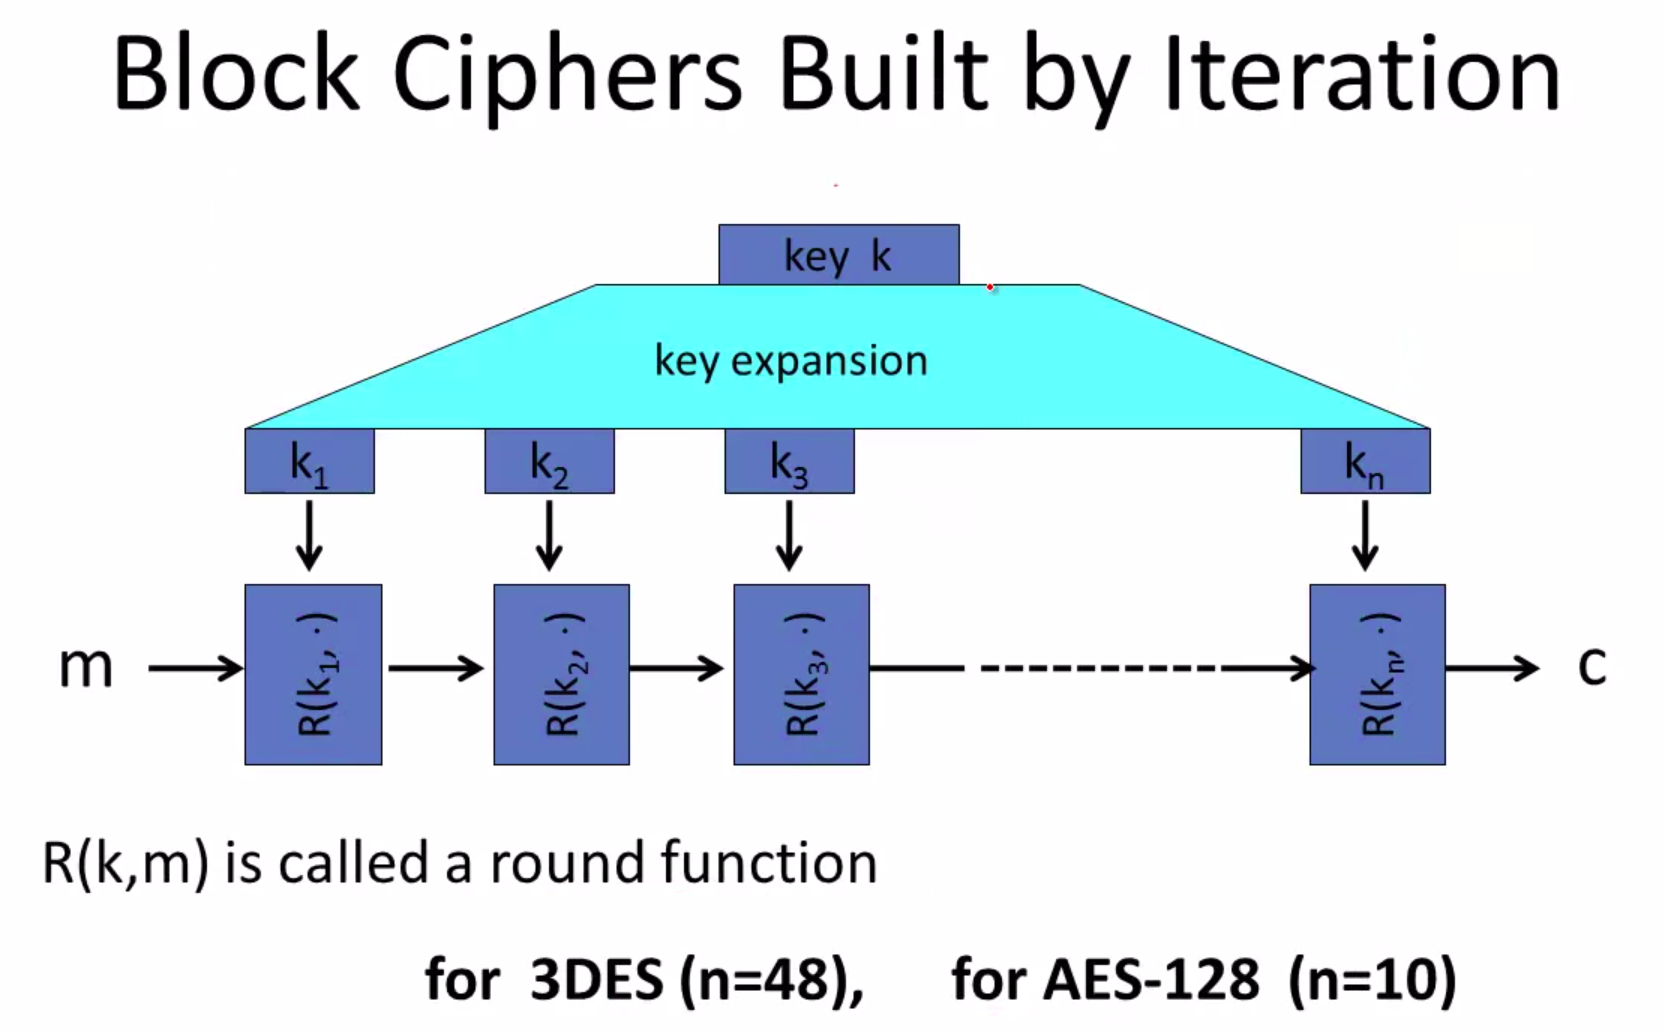
\includegraphics[width = 0.50\textwidth, center]{gfx/crypto/block-cipher.png}
    \caption{WEP Protocol}
\end{figure}

Block Ciphers are considerably slower than stream ciphers.

\begin{definition}[Pseudo Random Function]{}
    A Pseudo Random Function (PRF) defined over (K, X, Y) is $F: K \times X \rightarrow Y$, such that there exists an efficient algorithm to evaluate F(k, x).
\end{definition}

\begin{definition}[Pseudo Random Permutation]{}
    A Pseudo Random Permutation (PRP) defined over (K, X) is $F: K \times X \rightarrow X$, such that
    \begin{itemize}
        \item there exists an efficient algorithm to evaluate F(k, x).
        \item There exists function E(k, .) that is one-to-one. (i.e. given key, message to cipher is bijective)
        \item There exists an efficient inversion algorithm D(k, y).
    \end{itemize}
\end{definition}

A Pseudo Random Permutation is a Block Cipher, the terms might be used interchangably in different contexts.


\subsection{Data Encryption Standard (DES)}

56 bit key size, 64 bit block length. Widely used, but fell to complete search of the key.

For any functions $f_1, f_2, \dots, f_d: \{0, 1\}^n \rightarrow \{0, 1\}^n$.




\section{Message Authentication Codes}

The Goal is to maintain Integrity not Confidentiality.

\begin{definition}[Message Authentication Codes]{}
    Message Authentication Codes (MAC) $I = (S, V)$, defined over keyspace $\mathcal{K}$, message space $\mathcal{M}$, and tag space $\mathcal{T}$ is a pair of algorithms:
    \begin{itemize}
        \item $S(k, m) \rightarrow t \in \mathcal{T}$ outputs a tag.
        \item $V(k, m, t) \rightarrow \{true, false\}$ outputs a tag.
    \end{itemize}
    Such that $V(k, m, S(k, m)) = true \;\forall (k, m)$. 
\end{definition}

We shall define the goal of the attacker to be \textbf{Existential Forgery}, i.e. if we allow the attacker to sample several message tag pairs on messages of his choice $(m_i, t_i)\;i=1,2,\dots,q\;$, and we ask the attacker to produce a new message, tag pair not in the set of queries $(m^\prime, t^\prime) \notin \{(m_i, t_i)\;i=1,2,\dots,q\;\} \;\; \text{ such that } V(k, m, t) = true$, the advantage (i.e. the probability of successfully outputing a key-value pair) is negligible.

\begin{theorem}[Advantage against MAC]{}
    Given a MAC $I_F$ based on a Pseudo Random Function which outputs a tag of length |Y| being attacked by an adversary A is always less than that of it's Pseudo Random Function $F$ being attacked by adversary B summed with the inverse length of the tag.
    \begin{equation*}
        Adv_{MAC}[A, I_F] \leq Adv_{PRF}[B, F] + 1/|Y|
    \end{equation*}
\end{theorem}

\chapter{Binary Exploits}

\section*{Introduction}
Binary exploitation is the process of subverting a compiled application
t it violates some trust boundary in a way that is advantageous to you, 
the attacker.The exploits are explained breifly and then given case 
studies for it to be understood better.

\section{Buffer Overflow}
A buffer overflow occurs when a piece of data overflows the storage space
given to it. In these types of exploits, usually stack smashing occurs which 
changes value of non intended variables and helps in changing the flow of the 
program in some way.

\subsection{Stack}
One of the most important component to understand for binary exploitation and 
by extention buffer overflow is the stack. It is the location where all the 
variables and 
\setcounter{equation}{0}

\chapter{Systems and Exploitation}

\section*{Introduction}
The following chapter is an introduction to case studies of well knowns exploits, intoducing mobile systems and gaming consoles ( The easiest to hack, for their exploitation is mainstream). This is an introduction to the basics of actual life exploiting and will go into details on how the exploits were used, how to install them, their working and also how to replicate it. Specific systems will be covered in a one to one case based scenario. 

\section*{Terminology}
There are some very common terms encountered while browsing through this piece and also while refering to external resources specific to console exploitation (As I told you, it \textit{was} (is) very mainstream). Exploitation of systems with only a software is known as a softmod, whereas one done by physically modifying your hardware is known as hardmod. There are obvious advantages to both, a softmod is usually protected from in the next firmware update whereas hardmods are usually based on hardware vulnerabilities (But not always) and thus are harder to protect against after product is in the hands of the public.

\section{PSP}
One of the most exploited (\textit{Hacked}) system out there. It is the one that even I have reaped the benifits of, by doing \textit{legal} things, of course. It is also the one which I remember following to check out if the next version was exploitable, was it safe, did the risks outweigh the positives, etc. So here, I will explain how the PSP was exploited, why was it \textit{easy} and also replication.

\section{Android}
For android devices, it is not technically exploitaion as Android does not dissalow it, it is the OEMs which refuse access to root for customers. So rooting \textit{technically}, if the OEM ( like Xiaomi ) allows it, is not exploitaiton, but it does allow access to the complete system, so I am going to proceed with calling it exploitaiton of Android Rooting on android differs from phone to phone ( Or more like OEMs to OEMs ), and can be trivially easy or a fairly complicated process. But the general flow of work goes like this: Normal Device $\rightarrow$ Unlocking Bootloader $\rightarrow$ Installing a custom recovery $\rightarrow$ Installing a root manager ( Like magisk or SuperSU ) $\rightarrow$ Reboot $\rightarrow$ Rooted Android 

\subsection{Bootloader}
The bootloader in an android device is hidden and is not accessible to the normal user. It is locked by the OEM, so in order to access it, it has to be unlocked first. The method differs for every phone, and the details can be found on XDA Developers website\footnote[1]{xda-developers.com}. Bootloader is explained in detail in the Operating System section, but a brief understanding is that it is piece of code that points which OS ( More specifically the kernel\footnote[2]{Learn More} ) to load. So the bootloader, after being unlocked will allow us to load a custom OS ( Known as recovery ). This is a standalone OS which allows us to \textit{flash} a zip to the main partition.

\subsubsection{Unlocking the Bootloader}
TO DO

\begin{figure}
    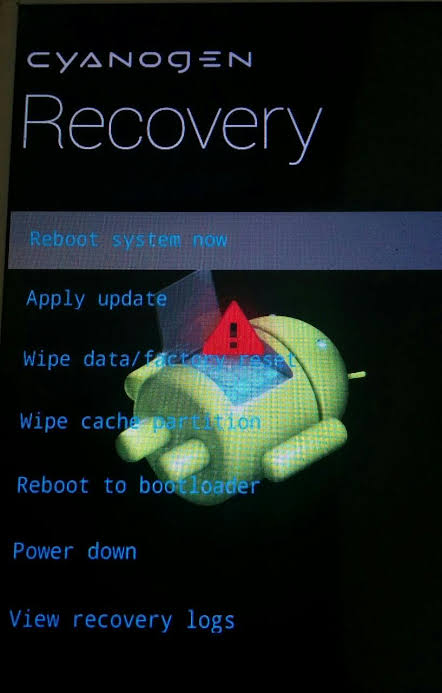
\includegraphics[width = 0.50\textwidth, center]{gfx/recovry.jpeg}    
    \caption{Recovery}
\end{figure}

\subsection{Recovery}
Recovery is an OS, which has a single purpose of allowing recovery. What it means is that it is a small OS which helps in fixing your main OS by providing tools to fix it ( Kind of like the live linux systems ). It is a minimal shell which allows for some fastboot and posix commands to run. It is most usefull in flashing zips which are either ROMs, custom kernels, or root binaries.The vanilla recovery that comes with the device does not allow for any such modifications, and this is where a custom recovery comes into picture. It allows for any modification and installation from within the recovery itself.

\subsubsection{Custom Recovery}
Custom recovery is the software which performs function of a recovery but allows for remote application i.e no need for another device to give commands to the system for it to work. One of the earlier custom recovery software was ClockworkMod which was one of the primary custom recovery for Android versions till 4.0, after which TWRP started to take over as the preferred recovery software.

\subsection{ADB and Fastboot}
ADB and Fastboot are utilities 

\subsubsection{Andoid Debugging Bridge}
Android Debugging Bridge ( known as ADB ) is a tool which allow for 
communication with an android device via USB. It is a shell with basic 
commands that allow a device to execute \textit{debug} commands. It is 
a basic version of a UNIX shell.

\begin{figure}
    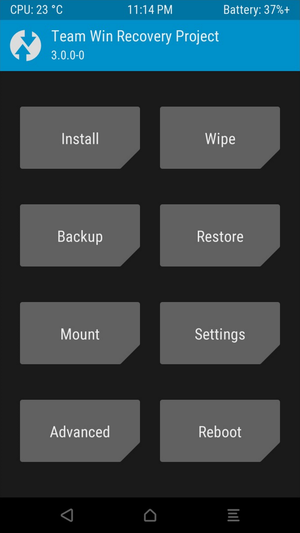
\includegraphics[width = 0.50\textwidth, center]{gfx/twrp.png}    
    \caption{TWRP}
\end{figure}
\cleardoublepage

\end{document}
